\documentclass{bioinfo}
\copyrightyear{2012}
\pubyear{2012}

\usepackage{subfig}
\usepackage{listings}
\usepackage{ifthen}

\lstset{language=Java,
morendkeywords={String, Throwable}
captionpos=b,
basicstyle=\scriptsize\ttfamily,%\bfseries
stringstyle=\color{darkred}\scriptsize\ttfamily,
keywordstyle=\color{royalblue}\bfseries\ttfamily,
ndkeywordstyle=\color{forrestgreen},
numbers=left,
numberstyle=\scriptsize,
% backgroundcolor=\color{lightgray},
breaklines=true,
tabsize=2,
frame=single,
breakatwhitespace=true,
identifierstyle=\color{black},
% morecomment=[l][\color{forrestgreen}]{//},
% morecomment=[s][\color{lightblue}]{/**}{*/},
% morecomment=[s][\color{forrestgreen}]{/*}{*/},
commentstyle=\ttfamily\itshape\color{forrestgreen}
% framexleftmargin=5mm,
% rulesepcolor=\color{lightgray}
% frameround=ttff
}

% MACROS:

\newcommand{\TODO}[1]{\textcolor{red}{\textbf{#1}}}
\newcommand{\AbstractDESSolver}{\texttt{Abstract\-DES\-Solver}}
\newcommand{\OverdeterminationValidator}{\texttt{Overdetermination\-Validator}}
\newcommand{\SBMLinterpreter}{\texttt{SBML\-interpreter}}
\newcommand{\FirstOrderSolver}{\texttt{First\-Order\-Solver}}
\newcommand{\AbstractIntegrator}{\texttt{AbstractIntegrator}}
\newcommand{\MultiTable}{\texttt{Multi\-Table}}
\newcommand{\Block}{\texttt{Block}}

\hyphenation{
  % TODO hypens for regular words
  im-ple-men-ta-tions
}

% some nice colors
\definecolor{royalblue}{cmyk}{.93, .79, 0, 0}
\definecolor{lightblue}{cmyk}{.10, .017, 0, 0}
\definecolor{forrestgreen}{cmyk}{.76, 0, .76, .45}
\definecolor{darkred}{rgb}{.7,0,0}
\definecolor{winered}{cmyk}{0,1,0.331,0.502}
\definecolor{lightgray}{gray}{0.97}

\begin{document}
\firstpage{1}

\title[Simulation Core Library]{Simulation Core Library: the Java
library for numerical computation in systems biology} \author[Dr\"ager
\textit{et~al.}]{%
Andreas Dr\"ager\,$^{1,*}$, Roland Keller\,$^{1}$, 
Alexander D\"orr\,$^{1}$,
Akito Tabira\,$^{2}$,
Akira Funahashi\,$^{2}$,
\TODO{%
Michael J. Ziller\,$^{3}$
Nicolas Rodriguez\,$^{4}$,
Nicolas Le Nov\`{e}re\,$^{4}$
Michael T. Cooling\,$^{4}$} and
Andreas Zell\,$^1$\footnote{to whom correspondence should be addressed}}
\address{$^{1}$Center for Bioinformatics Tuebingen (ZBIT), University of
Tuebingen, T\"ubingen, Germany\\
$^{2}$Keio University, Graduate School of Science and Technology, Yokohama,
Japan\\
\TODO{%
$^{3}$Department of Stem Cell and Regenerative Biology, Harvard University,
Cambridge, %MA, 
USA\\
$^{4}$European Bioinformatics Institute, Wellcome Trust Genome Campus,
Hinxton, %Cambridge, 
UK\\
$^{4}$Auckland Bioengineering Institute, University of Auckland, Auckland, New
Zealand}}

\history{Received on XXXXX; revised on XXXXX; accepted on XXXXX}

\editor{Associate Editor: XXXXXXX}

\maketitle

\begin{abstract}
\section{Motivation:}
Dynamic simulation of biological phenomenons belongs to the key aspects of
research in systems biology. Available implementations of numerical methods,
however, can often not easily be used as a backend in customized programs.
\section{Results:}
The Simulation Core Library is a community-driven project that provides a large
collection of numerical solvers and a sophisticated interface hierarchy for the
definition of custom differential equation systems. It is entirely
implemented in Java\texttrademark{} without the necessity to
include any platform-dependent wrappers or libraries, and does not depend on any
commercial library.
%, and can be used on every operating system for which a JVM
%is available.
It already includes an efficient and exhaustive implementation of methods to
interpret the content of models encoded in the SBML based on the JSBML project.
To demonstrate its capabilities, it has been benchmarked against the entire SBML
Test Suite and %also been used to simulate 
all models of the BioModels.net database.
\section{Availability:}
Source code, binaries, and documentation can be freely obtained under the terms
of the LGPL 3.1 from the website
\href{https://sourceforge.net/projects/simulation-core-library}{https://sourceforge.net/projects/simulation-core-library}.

\section{Contact:}
\href{mailto:andreas.draeger@uni-tuebingen.de}{andreas.draeger@uni-tuebingen.de}

\section{Supplementary information:}
% TODO: Provide additional material
Supplementary data is available at Bioinformatics online.

\end{abstract}

\section{Introduction}

Following the aim to make biological phenomena predictable, modeling, 
simulation, and computer analysis of biological networks has become an integral
part of modern biological research. XML-based standard description languages
such as the Systems Biology Markup Language (SBML, \citealt{Hucka2003}) or
CellML \citep{Lloyd2004} specify rich sets of methods for the interpretation
of biological network models in terms of a differential equation system with
additional elements such as events and rules.
Although libraries for reading and manipulating the information content of
these XML-based languages are available.
For model building, simulation, and calibration processes (e.g., the
estimation of parameter values), however, a multiple-purpose and 
efficient numerical solver library that has been designed with respect to the
requirements of biological network models is a crucial prerequisite.
The vast majority of available solvers for these systems is either
part of a larger software suite and can therefore not be easily integrated into
custom programs, or implemented in programing languages, which are either
platform-dependent or even require a commercial license for their
execution.

%The modeling language SBML (Systems Biology Markup Language,
%\citealt{Hucka2003}) constitutes an important \emph{de facto} standard for the
%exchange of biochemical network models.
%SBML defines a set of data structures and provides rules about how to interpret
%and simulate these kinds of models.

%Models in systems biology may combine an ordinary differential equation system,
%which is the basis for numerical simulation, with additional elements such as
%rules and events.  These elements further influence the system. 
%For instance,
%an event takes place if a certain trigger condition becomes true. Whenever this
%happens, event assignments may change the values of model components, such as
%parameter values or compartment sizes. Rules can directly assign new values to
%their objectives, e.g., the concentration of a reacting species.

There are several stand-alone programs (written in Java, C, or MATLAB) with
graphical user interfaces available that fulfil those important requests, for
instance, the Virtual Cell \citep{Loew2001}, iBioSim \citep{Myers2009},
PottersWheel \citep{Maiwald2008}, COPASI \citep{Hoops2006}, SBToolbox2
\citep{SBT_Schmidt2006}, or the Systems Biology Workbench with Roadrunner (SBW,
\citealt{Bergmann06}).
However, it is difficult to integrate the contained simulation routines into
other programs.
The SBML ODE Solver Library \citep{Machne2006}, which is written in C and based
on the libSBML library \citep{Bornstein2008},  provides such a simulation
routine. The SUNDIALS package is used for solving the differential equation
system given in the model.

In contrast to that we here present a platform-independent simulation API in
Java that interprets the content of such a model and predicts the dynamic
behavior of the model�s components. It is the first simulation routine which is
based on the Java library JSBML \citep{Draeger2011b}, a specifically
developed data structure to read and write models from and into SBML files and
to deal with their structure in memory. The API contains an interpreter for the
SBML model and several different ODE solvers. The generic library is completely
decoupled from any graphical user interface and can hence easily be integrated
as an API (Application Programming Interface) into third-party programs.

\TODO{Describe this as a potential application.}
The Simulation Core Library has already been integrated into the widely
used program CellDesigner version 4.2 \citep{Funahashi2003} as an internal simulation
library. The stand-alone application
SBMLsimulator\footnote{\url{http://www.cogsys.cs.uni-tuebingen.de/software/SBMLsimulator}}
provides a convenient graphical user interface for the simulation of SBML models
and uses this library as its computational backend.
%Secondly, a graphical and command-line user interface that provides
%a connection to the heuristic optimization framework EvA2 \citep{Kron10EvA2}.
% The combination of SBMLsimulator and EvA2 \citep{Kron10EvA2} estimates the values of all parameters with
%respect to given time-series of metabolite or gene expression values. 

\begin{methods}
\section{Implementation}
\begin{figure}
%\centerline{
%  \subfloat[Solvers.]{
%    \label{fig:Solvers}
%    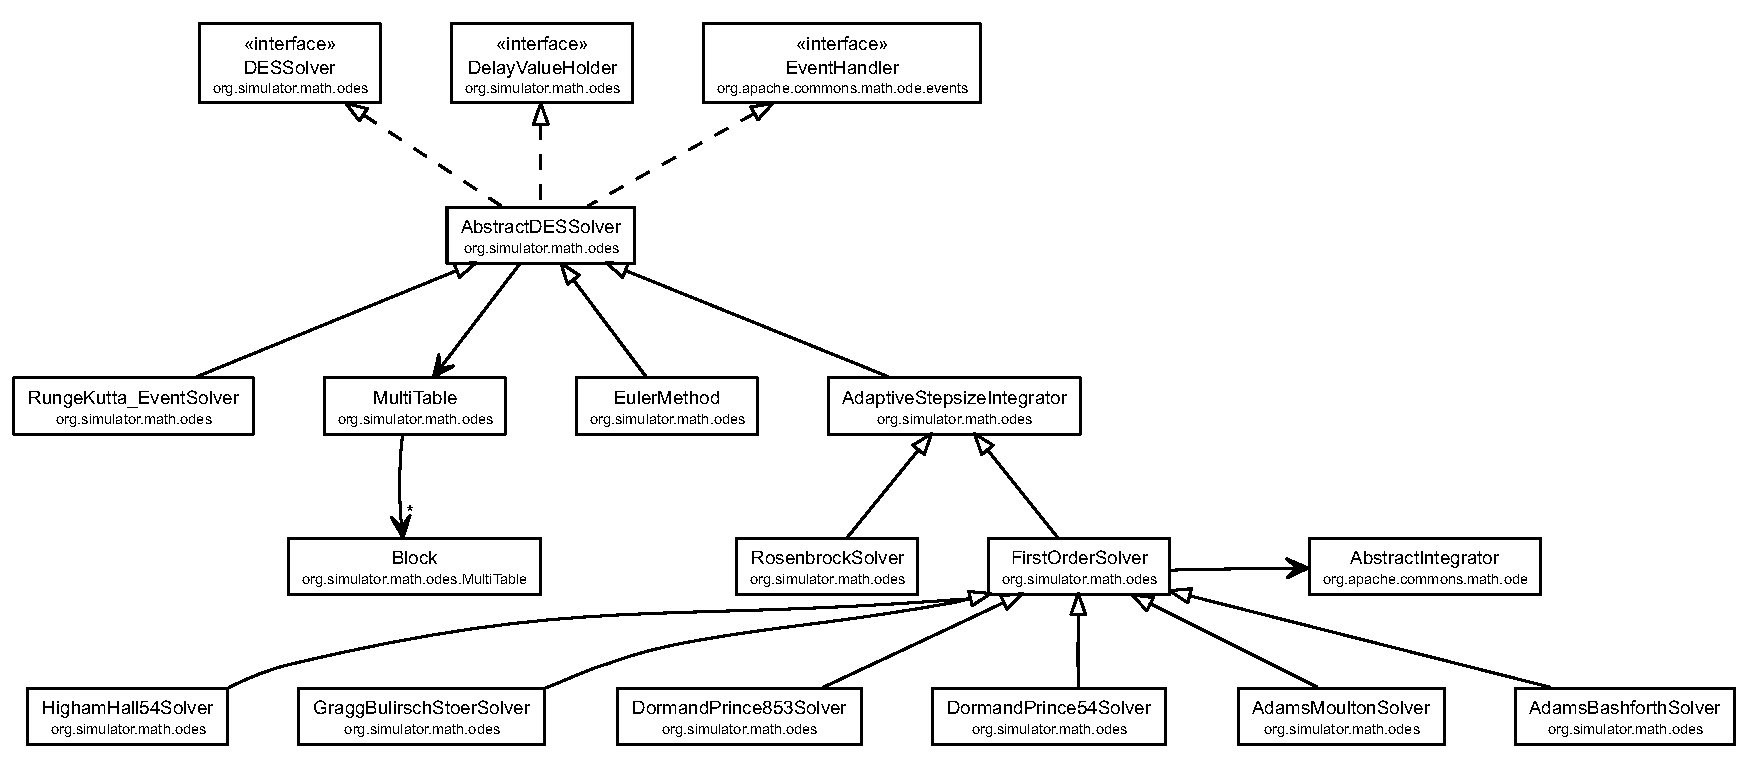
\includegraphics[width=.5\textwidth]{img/Solvers.pdf}
%  }
%  \hfill
%  \subfloat[Differential equation systems.]{
%    \label{fig:DESystems}
%    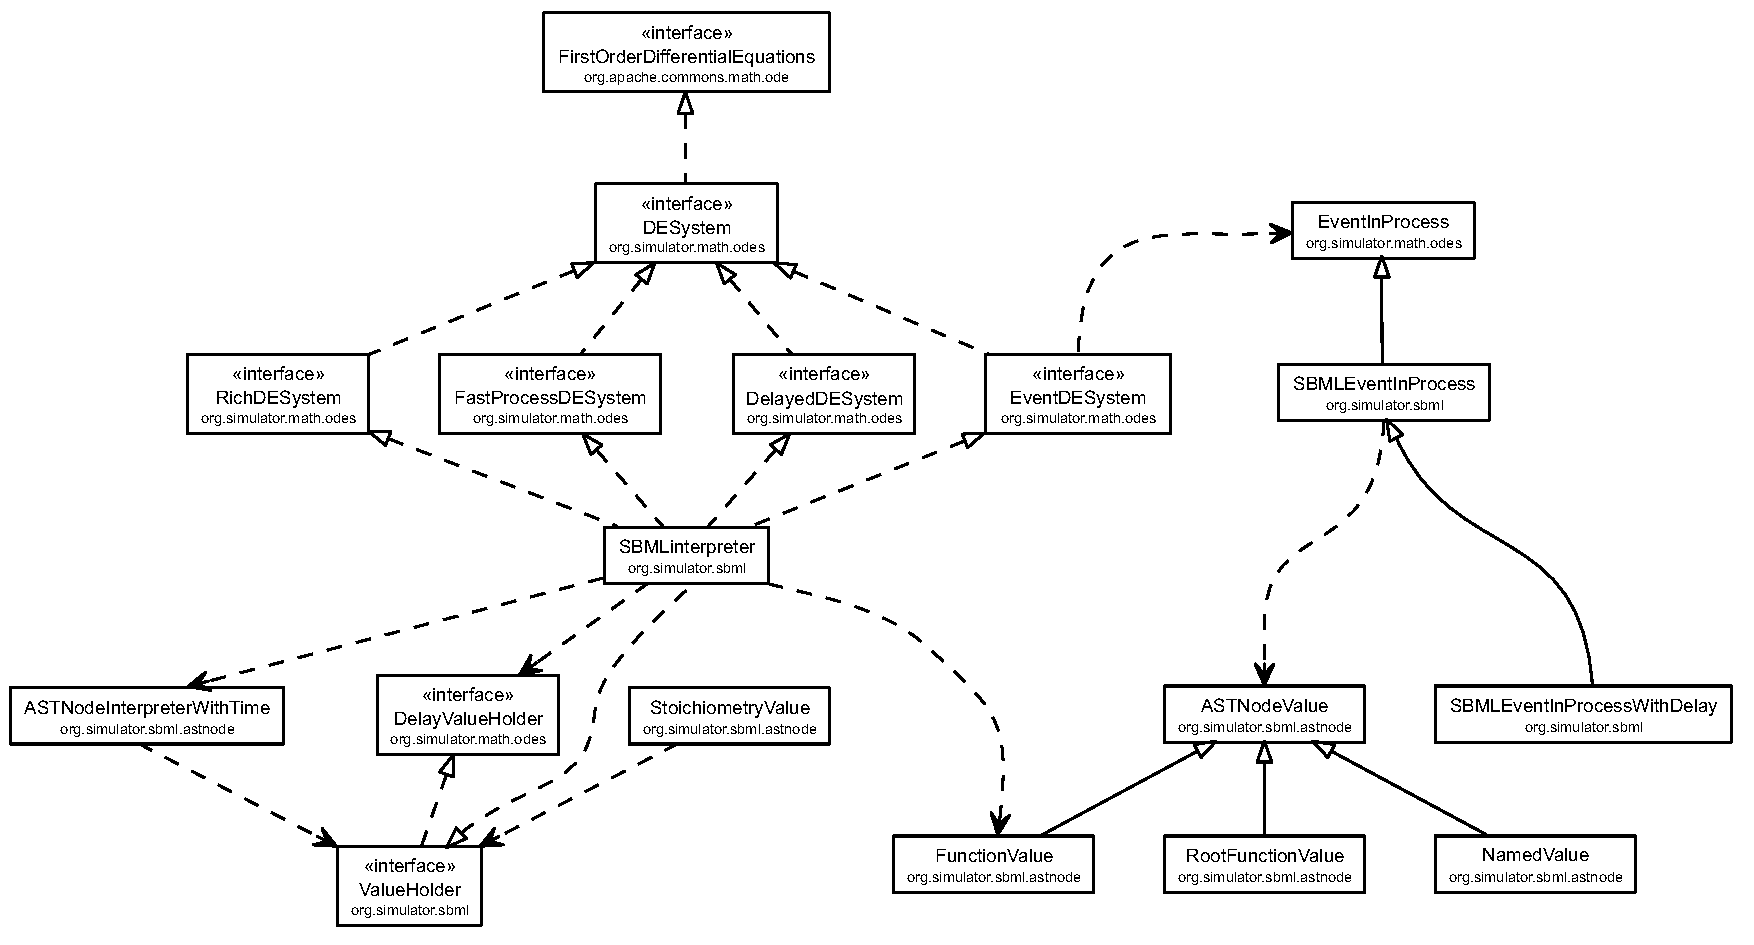
\includegraphics[width=.5\textwidth]{img/SBMLInterpreter.pdf}
%  }
%}
\centering{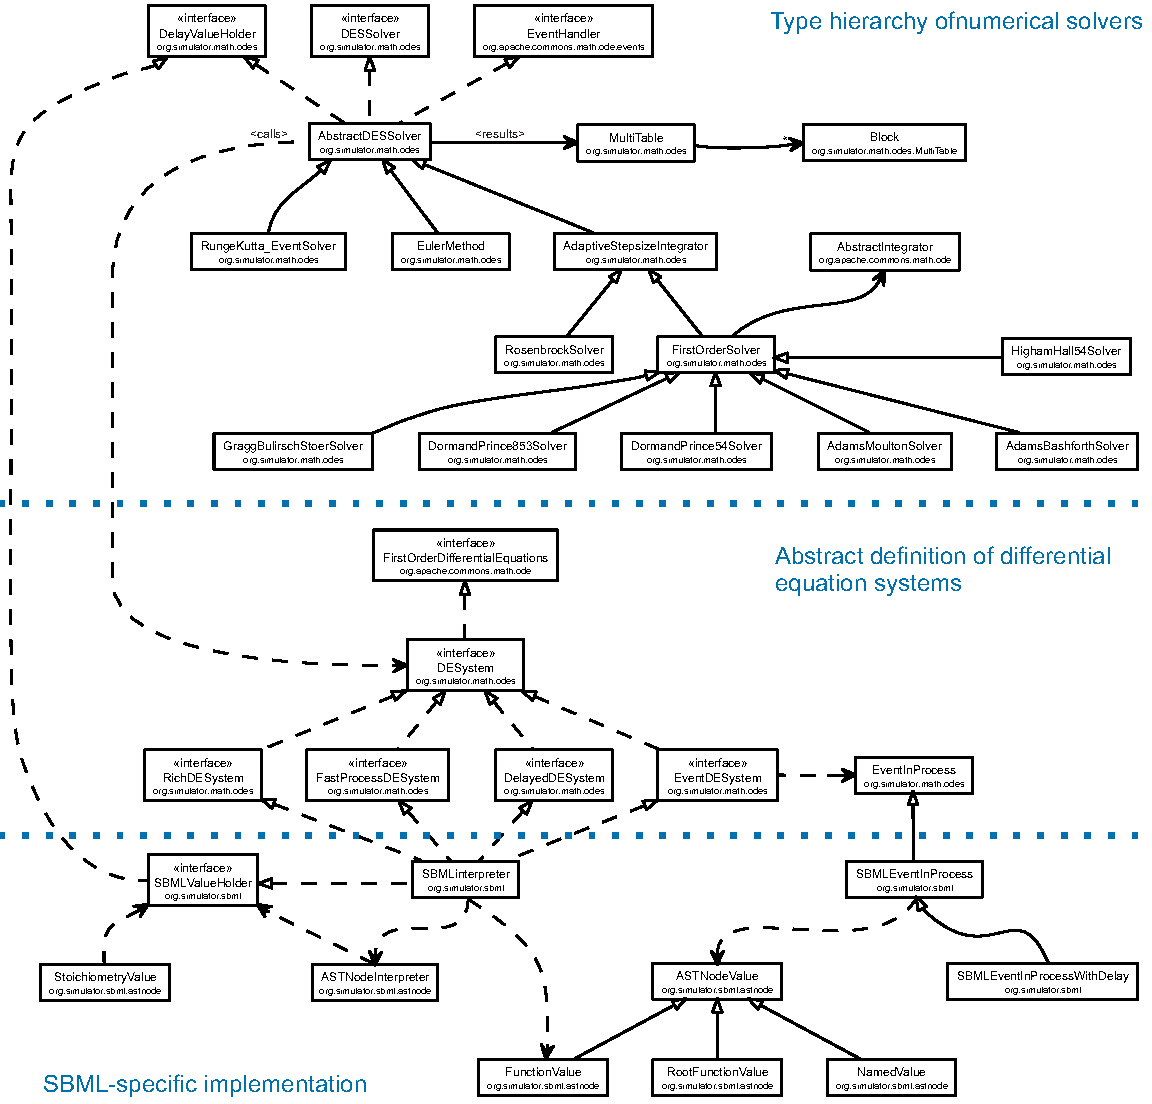
\includegraphics[width=.5\textwidth]{img/UML_Solvers_and_Systems.pdf}}
\caption[Architecture of the Simulation Core Library]{Architecture of
the Simulation Core Library (slightly simplified). Numerical methods are
strictly separated from differential equation systems. The upper part displays
the unified type hierarchy of all numberical integration methods, which are currently part of the
library, including solvers from Apache Commons Math library and Rosenbrock's
method. The class \MultiTable{} stores the results of a simulation within its
\Block{} data structures. The middle part shows the interfaces that
define several special types of the differential equations to be solved by the
numerical methods. This abstract description makes it possible to describe
various types of differential equation systems without directly linking it to a
particular type of biological networks. The class \SBMLinterpreter{} implements
all of these interfaces with respect to the information content of a given SBML
model. The interpreter causes the main run-time of the integration procedure.
This is why efficient and clearly organized data structures are required to
ensure a high performance of the overall library. The interpretation of SBML
models is therefore organized in the evaluation of events and rules, the
computation of stoichiometric information, and the computation of the current
values of all model components (such as species and compartments).
In this way it is possible to pass an instance of an interpreter for a
particular model system, such as SBML or CellML, to any available solver.}
\label{fig:Architecture}
\end{figure}
Fig.~\ref{fig:Architecture} displays the architecture of the library. All the
solver classes are derived from the abstract class \AbstractDESSolver.
Several solvers of the Apache Commons Math library are integrated with the help
of wrapper classes. Numerical methods and the actual differential equation
systems are strictly separated.

The class responsible for the evaluation of models encoded in SBML is
\SBMLinterpreter.
For a given value of the ODE system and a given time it returns the current set of
derivatives of the variables. It is connected to an efficient
interpreter for MathML expressions that are contained in kinetic laws, rules
and events. The nodes of the syntax tree of those expressions depend on the
current simulation time and the given values of the ODE system. If the time or
any of these values has changed, the value of the node has to be recalculated.
At the beginning of the simulation the syntax trees of all kinetic laws, rules
and events are restructured and merged to one large tree that contains
equivalent nodes only once. This leads to a decreasing computation time during
the simulation.

An extremely important aspect in the interpretation of SBML models is the
determination of the exact time at which an event occurs, as this can have a
high influence on the precision of the values of the system variables. We have
therefore adapted the Rosenbrock solver \citep{Kotcon2011}, which is an
integrator with an adaptive step size, to a very precise timing of the events.
Rosenbrock's method is well-suited even for stiff systems.

Algebraic rules are transferred to assignment rules before the simulation: One
of the variables contained in an algebraic rule is chosen as the variable of the
created assignment rule and the equation is solved by this variable. The
\OverdeterminationValidator{} in JSBML helps to ensure that no conflicts occur
between any of the chosen variables.

The simulation algorithm now proceeds as follows: In each time step the ODE
solver gets the current set of values of the variables as its initial values and
calculates the values for the next time point. After that events
and rules are processed, that can change the values. The calculated values are
then the initial values for the next time step. The event processing of the
Rosenbrock solver is different from that of the other solvers, as it
is directly integrated in the solver class and influences the adaptation of its
step size. This makes the processing of the events extremely precise.
\end{methods}

%\begin{table}[!t]
%\processtable{This is table caption\label{Tab:01}}
%{\begin{tabular}{llll}\toprule
%head1 & head2 & head3 & head4\\\midrule
%row1 & row1 & row1 & row1\\
%row4 & row4 & row4 & row4\\\botrule
%\end{tabular}}{This is a footnote}
%\end{table}


%%%%%%%%%%%%%%%%%%%%%%%%%%%%%%%%%%%%%%%%%%%%%%%%%%%%%%%%%%%%%%%%%%%%%%%%%%%%%%%%%%%%%
%
%     please remove the " % " symbol from \centerline{\includegraphics{fig01.eps}}
%     as it may ignore the figures.
%
%%%%%%%%%%%%%%%%%%%%%%%%%%%%%%%%%%%%%%%%%%%%%%%%%%%%%%%%%%%%%%%%%%%%%%%%%%%%%%%%%%%%%%

\section{Results and conclusion}
The SBML implementation has been successfully tested with the
SBML test suite (see
\href{http://sbml.org/Software/SBML_Test_Suite}{http://sbml.org/Software/SBML\_Test\_Suite}):
Rosenbrock's solver correctly simulates all models. In a further evaluation, it
solved nearly all (406 of the 409) models from the
\href{http://biomodels.net}{BioModels.net} database (release 21) \citep{Novere2006a}.

Therefore, the Simulation Core Library is an efficient Java tool for the
simulation of differential equation systems given in systems biology. It can be
easily integrated in larger applications, which display the simulation results
or optimize some parameters of ODE models. 

Besides its exisisting SBML implementation, the abstract program structure
supports the integration of other model formats such as CellML. To this end, it
is only necessary to implement a suitable interpreter class.

\section*{Acknowledgement}

The authors are grateful to Beky Kotcon, Samantha Mesuro, Daniel Rozenfeld, Anak
Yodpinyanee, Andres Perez, Eric Doi, Richard Mehlinger, Steven Ehrlich, Martin
Hunt, George Tucker, Peter Scherpelz, Aaron Becker, Eric Harley, and Chris
Moore, Harvey Mudd College, Claremont, California, USA, for providing an
Java implementation of Rosenbrock's numerical ODE solver.

\paragraph{Funding\textcolon} 
The Federal Ministry of Education and Research (BMBF, Germany) in the project
Virtual Liver Network (grant number 0315756).

\paragraph{Conflict of Interest\textcolon} none declared.

\bibliographystyle{natbib}
%\bibliographystyle{achemnat}
%\bibliographystyle{plainnat}
%\bibliographystyle{abbrv}
%\bibliographystyle{bioinformatics}
%
%\bibliographystyle{plain}
%
\bibliography{document}

\end{document}
